% 270 words
% Limit: 500 words
\section{Method}

\subsection{The data}

We crossmatched the \mct\ catalog of stellar rotation periods, measured from
\kepler\ light curves, with the \gaia\ DR2 catalog.
Reddening and extinction from dust was calculated for each star using the
Bayestar dust map implemented in the dustmaps {\it Python} package
\citep{green2018}.
We estimated effective temperatures from dereddened \Gaia\ \gcolor\ color,
using an 8th-order polynomial relation calibrated using .... stars
\racomment{ask Jason for details}.
\begin{equation}
    \mathrm{T_{eff}} = 8960 -4802C + 1931C^2 -2446C^3 + 2669C^4 - 1324C^5 +
    301C^6 - 26C^7,
% 8959.8112335205078, -4801.5566310882568, 1931.4756631851196,
%           -2445.9980716705322, 2669.0248055458069, -1324.0671020746231,
%           301.13205924630165, -25.923997443169355]
\end{equation}
where C is \gaia\ \gcolor.

\begin{figure}
  \caption{
A \gaia\ color magnitude diagram showing the \citet{mcquillan2014} sample with
    extinction-corrected magnitudes, colored by their rotation periods.
We excluded photometric binaries and subgiants from our analysis by removing
stars above the two dashed lines.
% The rotation periods of binaries and subgiants do not follow a Skumanich-like
% braking law.
% The rotation period gradient across the main sequence is visible by eye in
%     this figure: young, rapidly rotating stars are located below the old,
%     slowly rotating stars.
% since we rely on a simple scaling
% between rotation period and age to make the argument that the rotation period
% is not caused by incorrect period measurements.
}
  \centering
    \includegraphics[width=1\textwidth]{CMD_cuts}
\label{fig:CMD_cuts}
\end{figure}
To explore the age of this stellar population from a rotation-period
standpoint, it was first necessary to remove visual binaries and subgiants
from the sample.
The rotation-period evolution of these two types of stars is generally
different to that of single stars which more usually follow a Skumanich-like
spin-down law.
Tidal and magnetic interactions between the two components of a binary system
can influence the rotation periods of both stars, and the expanding envelopes
of subgiants drive rapid spin-down through conservation of angular momentum.
We removed visual binaries and subgiants from the sample by applying cuts to
the color-magnitude diagram (CMD), shown in figure \ref{fig:CMD_cuts}.
We fit a 6th-order polynomial to the main sequence and raised it by 0.22 dex,
to approximate the division between single stars and visual binaries.
We removed all stars above this line from the sample.
We removed subgiants by eliminating stars brighter than 6th magnitude in
\gaia\ G-band from the sample.
\begin{figure}
  \caption{
Dereddened main sequence stars with \mct\ rotation periods on the \gaia\ CMD
    with visual binaries removed.  Points are colored by their gyrochronal
    age, according to the
    \citet{angus2019} gyrochronology relation.
    A general age gradient is visible across the main sequence.
}
  \centering
    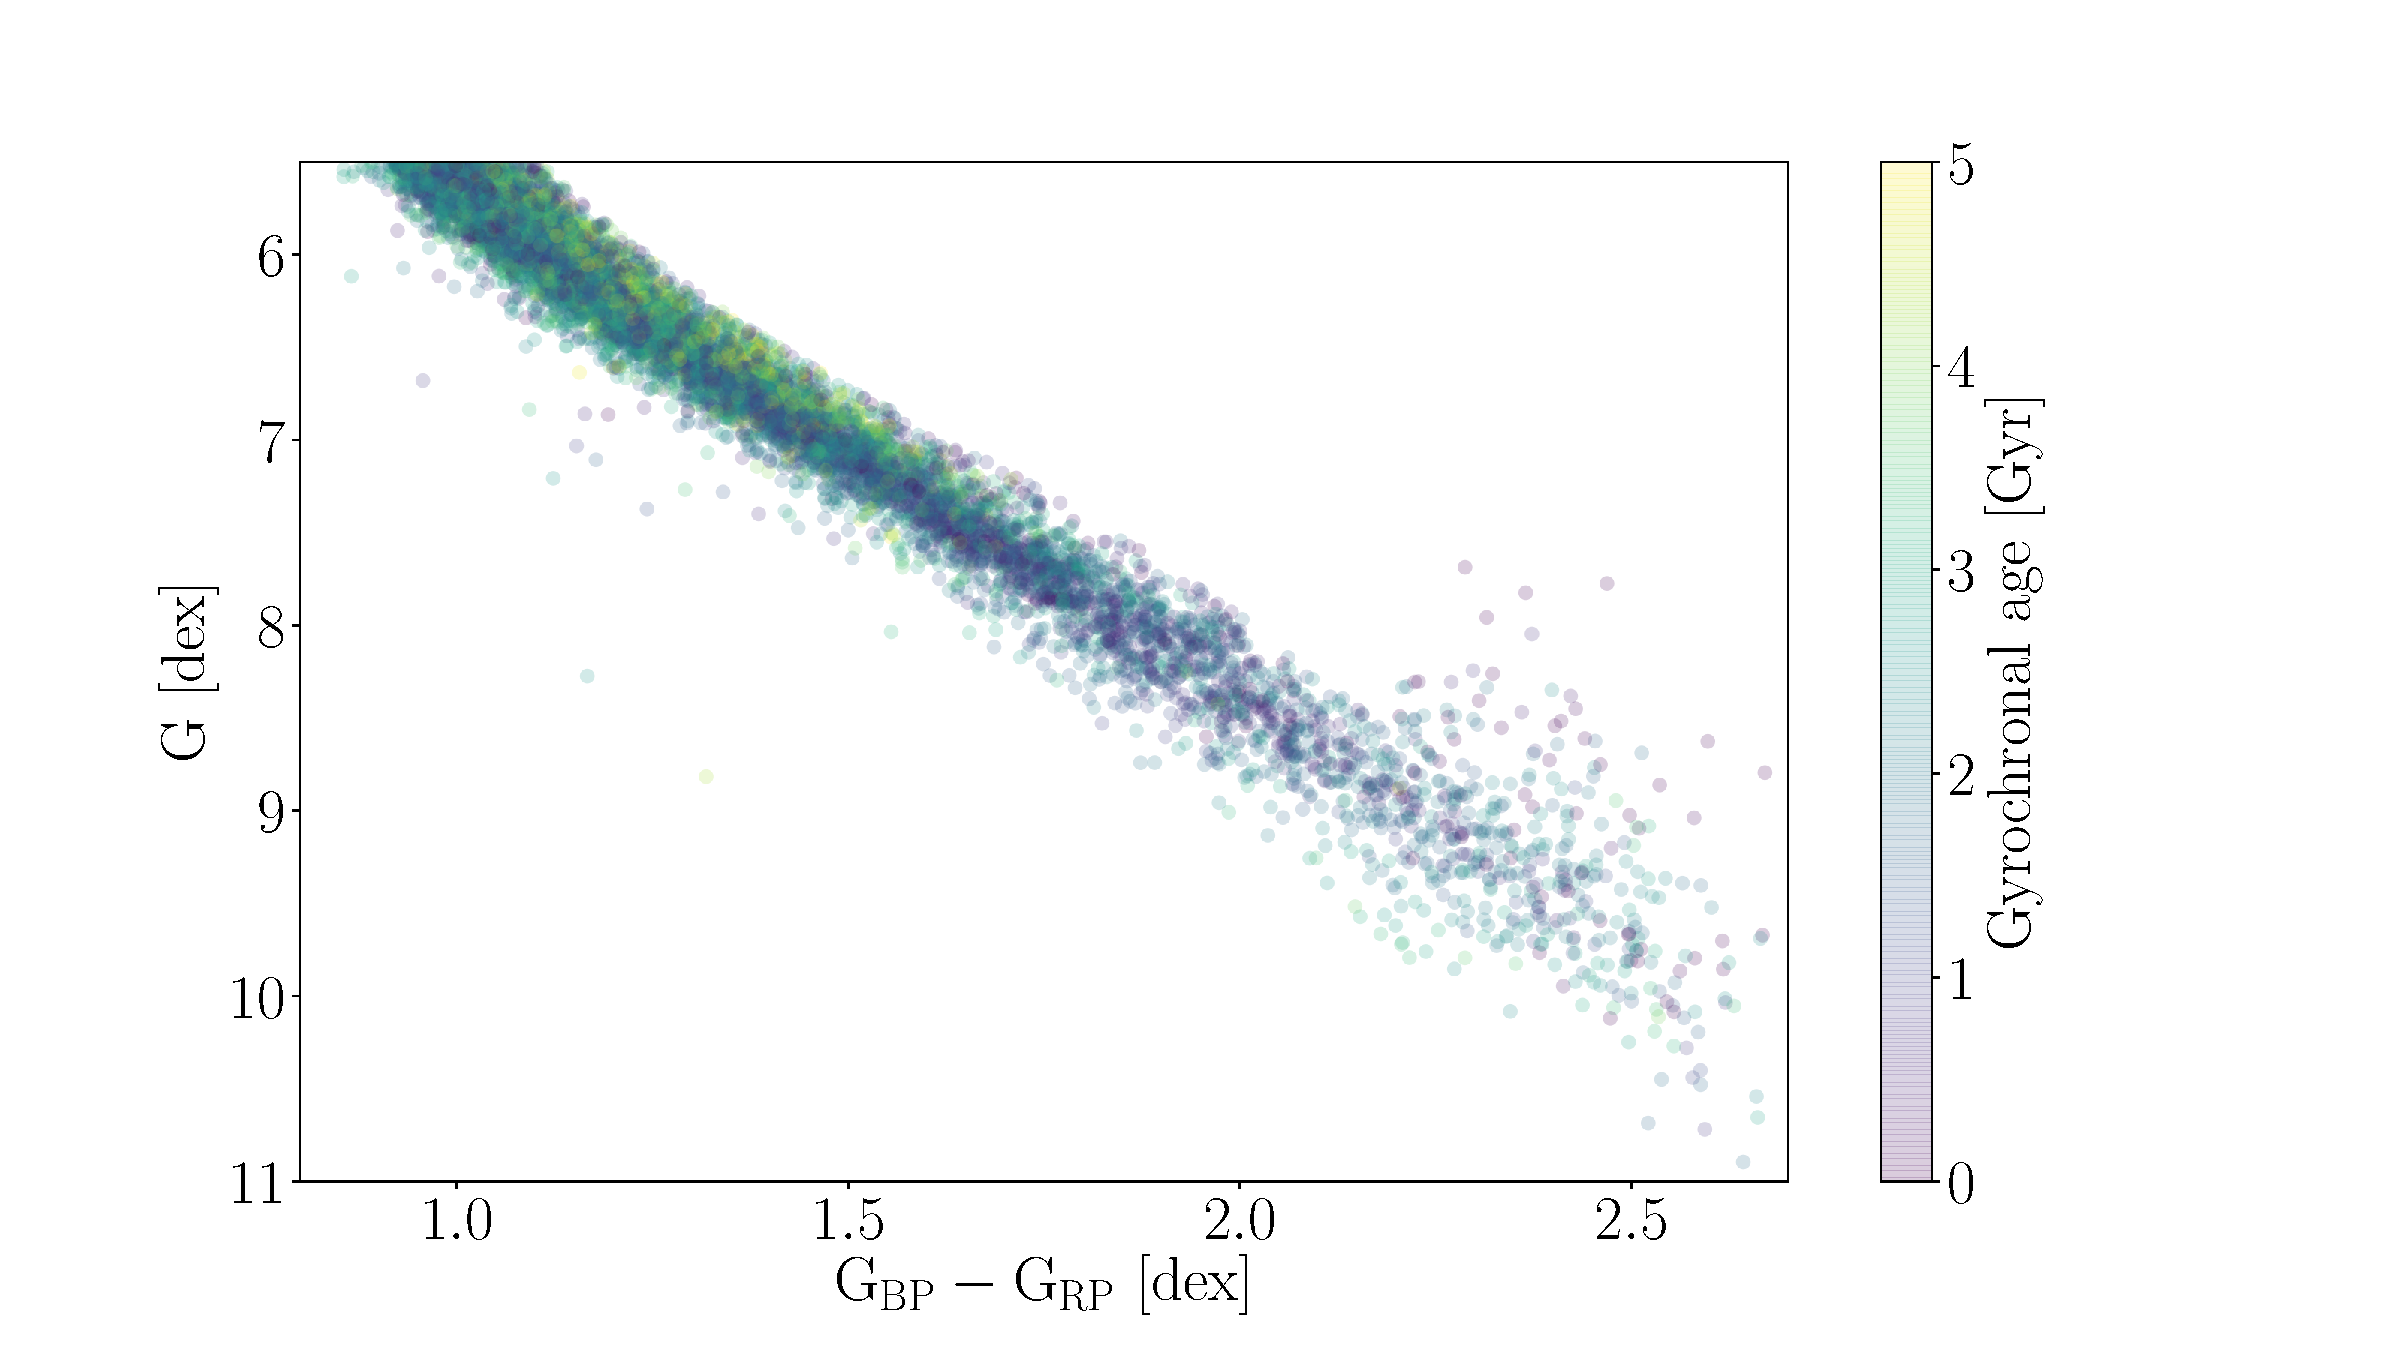
\includegraphics[width=1\textwidth]{age_gradient}
\label{fig:age_gradient}
\end{figure}

We removed stars with negative parallaxes and parallax signal-to-noise ratios
below 10 from the sample.
We also removed a small number of stars fainter than 16th magnitude from the
sample.
We used the {\tt Pyia} {\it Python} package to calculate stellar velocities.
{\tt Pyia} has built-in functionality for calculating velocity samples from
the full \gaia\ uncertainty covariance matrix via Monte Carlo sampling.
It therefore not only incorporates uncertainties on the \gaia\ positions
parallaxes and proper motions, it also accounts for the {\it covariance}
between these properties.
We removed stars with absolute \vb\ uncertainties greater than 1 \kms\ from
the sample.

% \begin{figure}
%   \caption{
% the rotation periods of stars in the \citet{mcquillan2014} sample vs.
% effective temperature.
% black points are dwarf stars identified as non-photometric binaries, hotter
% than 4800 k.
% blue circle points are non-photometric binary dwarfs, cooler than 4800 k, with
% a rotation period and \gaia\ color indicating they are older than 1.1 gyr.
% orange squares are stars that with rotation periods that fall just below the
% gap: they have rotation-ages between 0.5 and 1.1 gyrs.
% green triangles are stars with rotation periods faster than the main envelop
% of stars.
% these are probably binaries whose rotation periods are synchronized to their
% orbits and have been spun-up via tidal interactions.
% }
%   \centering
%     \includegraphics[width=1\textwidth]{period_teff}
% \label{fig:period_teff}
% \end{figure}
